% -----------------------------------------------------
\begin{figure*}[!t]
  \centering
  \fbox{%
    \parbox{0.95\textwidth}{%
      \centering
      \vspace{1cm}
      \textbf{[Placeholder for Benchmark Design Overview Figure]}
      
      \vspace{0.5cm}
      \small
      \textbf{Design notes:} This figure should illustrate the overall design of \textsc{XDomainBench}, including:
      \begin{itemize}[leftmargin=2cm,itemsep=0.1cm]
        \item Knowledge-composition space with two axes: Composition Order ($k$) and Mixture Structure (entropy)
        \item Session construction pipeline: from domain selection to multi-turn session generation
        \item Trajectory-level diagnostic annotations: difficulty trajectory ($\delta_t$) and domain-mixture trajectory ($w_t$)
        \item Interactive evaluation protocol: stateless, history, and memory-budget modes
        \item Example session structure showing turn coupling and cross-domain integration
      \end{itemize}
      \vspace{1cm}
    }%
  }
  \caption{Overview of \textsc{XDomainBench} design framework. The benchmark formalizes interdisciplinary reasoning through a controllable knowledge-composition space, generates interactive multi-turn sessions with trajectory-level diagnostic annotations, and evaluates models under standardized protocols.}
  \label{fig:bench_design}
  \vspace{-3mm}
\end{figure*}

\section{Benchmark Design}
\label{sec:bench_design}

\subsection{Overview and design principles}
\label{sec:bench_overview}

% -----------------------------------------------------

Figure~\ref{fig:bench_design} summarizes the overall design.
\textsc{XDomainBench} is a \emph{diagnostic} benchmark for \emph{interactive interdisciplinary scientific reasoning}, where the unit of evaluation is a multi-turn \emph{session} rather than a single query.

\paragraph{Design goals.}
We target three goals: (i) \textbf{Controllability:} formalize cross-domain reasoning as a \emph{knowledge-composition space} with explicit controls over domain count and mixture evolution; (ii) \textbf{Evaluability:} ensure each turn admits a checkable target (exact match / structured parsing / judge scoring); (iii) \textbf{Diagnosability:} attach trajectory-level metadata to connect performance degradation to interpretable failure mechanisms~\citep{liang2022helm,ribeiro-etal-2020-beyond,kiela-etal-2021-dynabench,schlangen-2021-targeting}.

\paragraph{What a session looks like.}
A session is a sequence of turns $\{(x_t, y_t)\}_{t=1}^{T}$, where each turn provides a user query $x_t$ and a reference target $y_t$.
Turns are \emph{coupled}: later turns may reuse intermediate results, introduce new constraints, or require reconciliation across domains.

\begin{figure}[t]
  \centering
  \fbox{%
    \parbox{0.95\linewidth}{%
      \centering
      \vspace{1cm}
      \textbf{[Placeholder for Session Example and Output Format]}
      
      \vspace{0.5cm}
      \small
      \textbf{Design notes:} This figure should show:
      \begin{itemize}[leftmargin=0.5cm,itemsep=0.1cm]
        \item \textbf{Left:} Multi-turn session example (2-4 turns) showing turn coupling, cross-domain integration, input/output formats, domain mixture, and difficulty trajectory
        \item \textbf{Right:} Output format schemas for different task types (Factual QA: exact match; Derivation: numeric result + justification; Structured: JSON with predefined keys; Long-form: judge-based scoring)
      \end{itemize}
      \vspace{1cm}
    }%
  }
  \caption{Example multi-turn session and output format schemas in \textsc{XDomainBench}.}
  \label{fig:session_example}
  \vspace{-3mm}
\end{figure}

% 这里补一个"真实session示例"（2-4 turns）的小表或listing。如果篇幅不够，甚至是放"单个 turn 的例子"可以对不重要的文字用...，只：输入：一句话描述（省略背景）输出：一个很短的 JSON/最终答案形式。但是必须要有。

% ==========================================================
\subsection{Knowledge-composition space}
\label{sec:composition_space}

We formalize interdisciplinary reasoning via a controllable \emph{knowledge-composition space}.
A session draws from a set of domains $\mathcal{D}=\{d_1,\ldots,d_k\}$, where $k$ is the \emph{composition order} (session-level dimensionality).
At each turn $t$, we specify a \emph{target domain-mixture distribution} $w_t^{\text{target}} \in \Delta^{k-1}$ over the selected domains, which governs how strongly the turn should rely on each domain.

\paragraph{Axis 1: composition order (how many domains).}
The composition order $k$ controls the number of distinct domains involved in a session.
Higher $k$ increases the space of coupled constraints and typically requires more integrative reasoning, consistent with known challenges in compositional generalization~\citep{lake2018generalization,keysers2020measuring}.

\paragraph{Axis 2: mixture structure (how domains are mixed).}
We quantify per-turn mixture dispersion using entropy:
\begin{equation}
H(w_t^{\text{target}}) = -\sum_{i=1}^{k} w^{\text{target}}_{t,i}\log w^{\text{target}}_{t,i}.
\end{equation}
Higher entropy corresponds to more balanced mixtures, while lower entropy corresponds to more concentrated mixtures.

\paragraph{Mixture drift across turns.}
We measure drift between consecutive turns using Jensen--Shannon divergence:
\begin{equation}
\mathrm{JSD}(w_t^{\text{target}} \,\|\, w_{t+1}^{\text{target}}).
\end{equation}
Drift and volatility statistics define representative mixture regimes (stable, gradual shift, abrupt shift, high-volatility).
Details are in Appendix~\ref{app:composition_metrics}.

\paragraph{Optional control: domain distance.}
We optionally control domain distance using semantic embeddings and cosine similarity to probe transfer difficulty~\citep{kashyap2021domain}.
% domain distance的定义与实现（例如，对domain描述做embedding然后算cosine距离？）。
Details are in Appendix~\ref{app:composition_metrics}.

\paragraph{Target vs.\ realized mixtures (validation).}
We distinguish the \emph{target} mixture $w_t^{\text{target}}$ (specified during instantiation) from a \emph{realized} estimate $w_t^{\text{realized}}$ (computed post hoc for validation).
We estimate $w_t^{\text{realized}}$ using a hybrid pipeline combining LLM analysis, lexical checks, and embedding-based tests~\citep{zheng-etal-2023-judging,laskar-etal-2024-systematic,reimers-gurevych-2019-sentence}.
Tolerance constraints ensure the realized trajectory matches the target regime (Appendix~\ref{app:signals}).
% 之前的版本里"$\{w_t\}$ is defined during session instantiation to realize a target mixture regime (e.g., stable, gradual shift, or fluctuation)"。那就是，构造时我们有一个目标轨迹，生成完又做了验证。所以，w_t^{target}：构造时预先指定的混合权重（我们控制的东西）。w_t^{realized}：生成后用某种方法估计/判定"这个 turn 实际更像哪些域"得到的权重（我们用于 audit 的东西）。所以，w_t^{realized} 的估计方法（LLM rubric / lexical / embedding分类器），以及容忍阈值（tolerance constraints）怎么设定？

% ==========================================================
\subsection{Tasks and domains}
\label{sec:tasks_domains}

\paragraph{Domains.}
\textsc{XDomainBench} covers 20 scientific domains across four categories: \textbf{Natural Sciences} (Biology, Chemistry, Physics, Earth Science), \textbf{Engineering} (Materials Science, Mechanical Engineering, Electrical Engineering), \textbf{Mathematics and Computing} (Mathematics, Computer Science, Statistics), and \textbf{Social Sciences and Humanities} (Economics, Psychology, Philosophy).
This spans closely related domains (e.g., Chemistry--Materials Science) and distant ones (e.g., Physics--Economics).
% 20个domain的名称列表，以及选择标准（例如：覆盖生命科学/物质科学/工程/数学/计算等；以及每个domain的来源语料/知识边界）。这是你的主要做的内容，或许你觉得太多放到附录里，但是它必须要在正文里有，现在太虚了。而且最好同时给每个domain的数据量（turn数或session数）以便在正文汇报平衡性。一般的benchmark中会把做成一个多层的圆形图。
Complete domain list, per-domain statistics, and selection criteria are in Appendix~\ref{app:dataset_stats}.

\paragraph{Task taxonomy.}
We categorize turns into four task types: \textbf{Factual QA} (direct knowledge recall), \textbf{Derivation} (step-by-step reasoning for numerical results), \textbf{Synthesis} (cross-domain integration), and \textbf{Analysis} (interpretation and comparison).
%四类任务的名字与精确定义（输入输出格式等可以放到附录里）。每类任务的占比/数量。
Each task type has a template family and domain-specific seed pools.
Task distributions and detailed schemas are in Appendix~\ref{app:dataset_stats}.



\paragraph{Turn format and required outputs.}
Each turn specifies a required output schema: exact match for factual QA, JSON for structured predictions, numeric result + justification for derivations.
Format violations are treated as \emph{ParseFail} (Appendix~\ref{app:nonanswer}).
%% 实际使用的输出schema（比如JSON字段名、是否要求前缀等），否则正文无法写得具体可复现。还是和上面一样，可以给一个最好看的，最小规模的例子。其余的细节再放到附录。








% ==========================================================
\subsection{Session construction and QA evaluability}
\label{sec:episode_construction}

\paragraph{Session blueprint.}
To construct a session, we sample: (i) a domain set $\mathcal{D}$ of size $k$; (ii) a target mixture regime $\{w_t^{\text{target}}\}_{t=1}^{T}$; and (iii) a difficulty regime $\{\delta_t\}_{t=1}^{T}$ (detailed in Sec.~\ref{sec:diagnostic_signals}).
We then generate turn prompts from task templates and domain-specific seed pools, ensuring turns are \emph{integrative}: later turns depend on earlier results, introduce cross-domain constraints, or require reconciliation across domains.

\paragraph{Ensuring evaluability and reducing ambiguity.}
We filter out prompts without stable, checkable targets.
Each turn uses one of: (i) exact match (EM) for factual QA; (ii) structured JSON/canonical forms for derivation/synthesis; (iii) judge-based scoring for complex analysis.
% turn里三类reference分别占比多少？哪些任务用EM，哪些用parser，哪些用judge？以及parser的规范（canonicalization规则）是否存在。
Filtering rules, canonicalization, and reference type distributions are in Appendix~\ref{app:dataset_construction} and Appendix~\ref{app:scoring}.

\paragraph{Reference answer curation and auditing.}
We curate reference answers using a hybrid approach: LLM-assisted generation, expert review for critical cases, and cross-annotation agreement checks~\citep{li2024arenahard,zhou2023instruction}.
%% 最最最最重要的：reference答案的来源（人工/LLM/混合）、审核流程（几位annotator、仲裁规则）、一致性统计（agreement）。如果你做了我们之前说的，有抽样地找人工专家评估，在这里要提到。
We implement safeguards against benchmark leakage and contamination~\citep{deng-etal-2024-investigating}.
Details are in Appendix~\ref{app:data_quality}.






% ==========================================================
\subsection{Trajectory-level diagnostic annotations}
\label{sec:diagnostic_signals}

A key goal of \textsc{XDomainBench} is to diagnose \emph{why} interdisciplinary reasoning degrades under high-dimensional compositions.
Thus, each session includes trajectory-level metadata for downstream analysis.

\paragraph{Difficulty trajectory.}
We attach a per-turn difficulty score $\delta_t$ as diagnostic metadata to analyze whether performance collapses are associated with specific difficulty regimes.
We estimate $\delta_t$ using a hybrid approach: (i) performance-based signals from a fixed pilot model ensemble (to avoid circular reasoning) and (ii) semantic complexity proxies.
%% δ_t 的范围/含义、估计方法（pilot模型集合？人标？复杂度proxy？）、以及如何保证不会"用被测模型定义难度"导致循环论证。
%% 是否δ_t 与人类难度标注/或与多模型平均正确率的相关系数？（哪怕抽样）。
We validate $\delta_t$ against human annotations and multi-model accuracy, reporting correlations in Appendix~\ref{app:trajectory_annotation}.

\paragraph{Domain-mixture trajectory.}
Each turn carries the target mixture $w_t^{\text{target}}$ (Sec.~\ref{sec:composition_space}).
We validate a realized estimate $w_t^{\text{realized}}$ post hoc to ensure turns match the intended regime.
Tracking $\{w_t^{\text{target}}\}$ enables analyses of mixture drift and its association with long-context failures, error accumulation, and memory contamination~\citep{bai-etal-2024-longbench,liu-etal-2024-lost}.
Validation procedures are in Appendix~\ref{app:signals}.

\paragraph{Pattern taxonomy (used in mechanism analysis).}
For mechanism-oriented diagnosis (Sec.~\ref{sec:mechanism}), we group sessions into pattern types based on difficulty and mixture drift/volatility statistics.
Patterns include: \textbf{stable} (low drift/volatility), \textbf{gradual shift} (monotonic drift), \textbf{abrupt shift} (high drift at specific turns), and \textbf{high-volatility} (high volatility throughout).
%% 需要你提供：你们最终用了哪些pattern类型（把附录里的名称和形式化定义，可以不把那几个公式搬过来，而是要给出定义），以及每类pattern的数量分布。
Formal definitions and distributions are in Appendix~\ref{app:pattern_taxonomy}.




% ==========================================================
\subsection{Standardized interactive evaluation protocol (reference controller)}
\label{sec:protocol}

\textsc{XDomainBench} evaluates models under a standardized interactive protocol to reduce prompt-engineering variance.
The protocol defines: (i) context visibility at each turn, (ii) output formatting for scoring, and (iii) memory management under budget constraints.

\paragraph{Interaction modes.}
We support three modes: \textbf{Stateless} (current turn only), \textbf{History} (full dialogue context), and \textbf{Memory budget} (bounded context via truncation/summarization).
This aligns with standard long-context evaluation settings~\citep{bai-etal-2024-longbench,liu-etal-2024-lost}.

\paragraph{Reference controller and format constraints.}
We provide a lightweight reference controller that structures each turn into an action--reasoning cycle to stabilize outputs~\citep{yao2023react,schick2023toolformer}.
The controller enforces output schemas for automatic parsing and scoring.
Invalid outputs are counted as \textbf{ParseFail}; refusals/empty answers as \textbf{NA}.
%% controller的核心prompt模板（system+user格式），依旧，最小化。
Details are in Appendix~\ref{app:controller}.

\paragraph{Default settings used in experiments.}
Unless otherwise specified, we report results under \textbf{History} mode (full dialogue context) with no explicit memory budget constraints.
%% 模式（stateless/history/memory budget） setting with a context window budget of %% tokens and a summarization strategy of %% .
%% 实验到底用哪个默认模式。
Protocol sensitivity analyses are in Appendix~\ref{app:controller}.


%这个图在之前的论文中也没有用到，而且它的信息密度低，可以用\algorithm来表达，或者直接放在附录里。
% \begin{figure*}[t] 
%   \centering
%   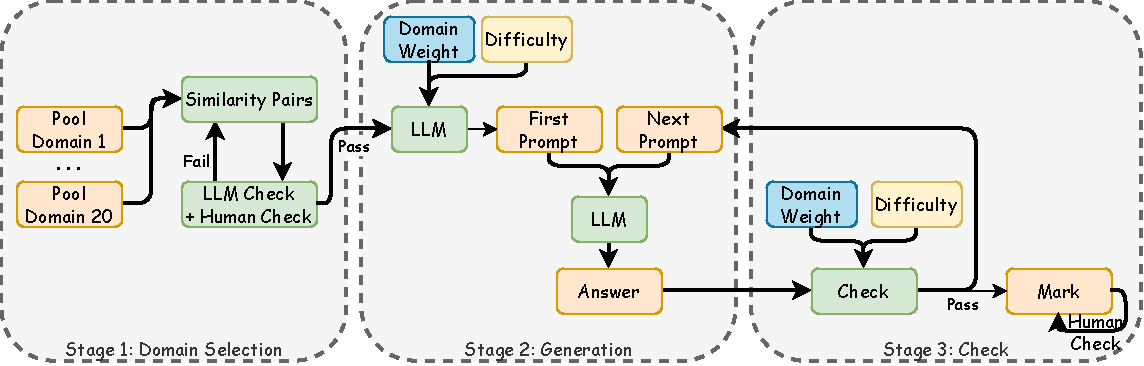
\includegraphics[width=\textwidth]{figures/Fig2.pdf}
%   \caption{Design of \textsc{XDomainBench}. We parameterize high-dimensional cross-domain reasoning as a controllable knowledge-composition space and generate realistic interactive sessions with trajectory-level diagnostic annotations.}
%   \label{fig:bench_design}
%   % \vspace{-3mm}
% \end{figure*}
% % -----------------------------------------------








% \subsection{Overview and design principles}
% \label{sec:bench_overview}
% AI4S increasingly relies on LLMs for knowledge synthesis, integrative reasoning, and interactive scientific assistance. However, interdisciplinary settings remain under-evaluated due to cross-domain data scarcity and the difficulty of reliable assessment at scale~\citep{zhang-etal-2024-comprehensive-survey,zheng-etal-2025-automation}.
% \textsc{XDomainBench} is a \emph{diagnostic} benchmark for \emph{interactive interdisciplinary scientific reasoning}, in which the unit of evaluation is a multi-turn \emph{interactive session}, where models must maintain consistency across evolving constraints and reuse intermediate results.
% Following widely adopted evaluation principles that emphasize controlled factors, robustness-aware stress testing, and mechanism-oriented analysis~\citep{liang2022helm,chang-etal-2023-survey,ribeiro-etal-2020-beyond,kiela-etal-2021-dynabench,schlangen-2021-targeting,zhu-etal-2023-promptrobust}, we formalize interdisciplinary reasoning through a controllable \emph{knowledge-composition space} and attach trajectory-level diagnostic signals for detailed downstream analysis.

% % -------- Figure placeholder (two-column) --------
% \begin{figure*}[t]
%   \centering
%   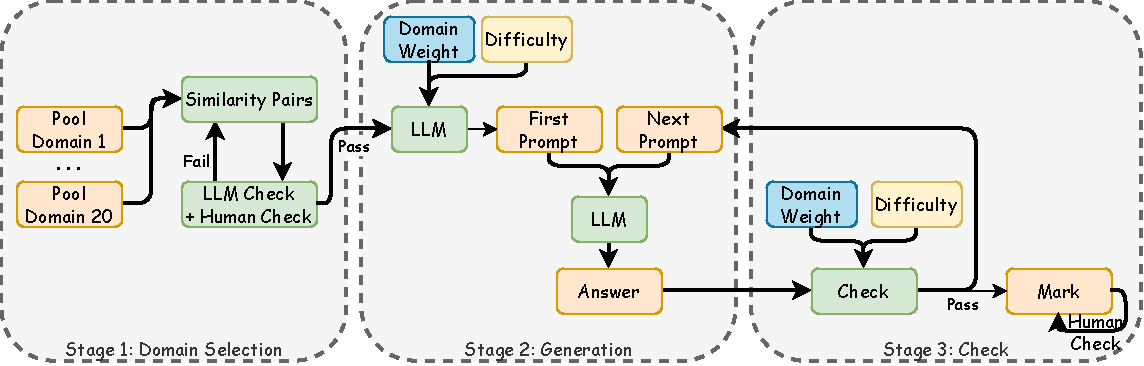
\includegraphics[width=\textwidth]{figures/Fig2.pdf}
%   \caption{Design of \textsc{XDomainBench}. We parameterize high-dimensional cross-domain reasoning as a controllable knowledge-composition space and generate realistic interactive sessions with trajectory-level diagnostic annotations.}
%   \label{fig:bench_design}
%   % \vspace{-3mm}
% \end{figure*}
% % -----------------------------------------------

% \subsection{Knowledge-composition space}
% \label{sec:composition_space}

% We define a session involving a domain set as $\mathcal{D}=\left\{d_1,\ldots,d_k\right\}$, and two primary axes that \emph{continuousize} cross-domain settings.
% % 
% % \subsubsection{Composition order}
% The \emph{composition order} or session-level dimensionality, $k$, is the number of distinct domains participating in a session.
% Increasing $k$ expands the combinatorial space of constraints and the need for systematic recombination, which is closely aligned with known challenges in compositional generalization~\citep{lake2018generalization,keysers2020measuring}.

% % \subsubsection{Mixture structure}
% Beyond the number of domains presented, we characterize how domains are combined at each turn as the \emph{turn-level domain mixture}.
% We represent the mixture at turn $t$ as a distribution $w_t \in \Delta^{k-1}$ over the selected domains, and summarize mixture structure using entropy: 
% \[
% H(w_t) = -\sum_{i=1}^{k} w_{t,i}\log w_{t,i}, 
% \]
% which is a standard measure of dispersion and uncertainty~\citep{shannon1948}.
% To quantify turn-to-turn \emph{mixture drift}, we use symmetric distributional distances such as Jensen--Shannon divergence~\citep{lin1991divergence}.
% We also allow optional controls over domain distance, which is %(e.g., selecting domain pairs with less or more distance), 
% consistent with prior work that identifies domain divergence as a meaningful factor in cross-domain transfer~\citep{kashyap2021domain}. We provide implementation details and calibration choices in Appendix~\ref{app:composition_metrics}.

% \subsection{Session construction pipeline and data quality}
% \label{sec:episode_construction}
% \textsc{XDomainBench} is designed to construct sessions that require \emph{integrative} cross-domain reasoning, rather than simple topic switching.
% We first build domain-specific seed pools and instantiate a target point in the knowledge-composition space (specified by order $k$ and mixture regime). Then, we generate a coherent multi-turn session with heterogeneous query forms (e.g., factual checking, derivations, synthesis, and code-like reasoning), reflecting realistic %scientific assistance 
% scenarios.
% While 
% Compared to existing science-oriented benchmarks~\citep{lu2022learn,rein2024gpqa}, \textsc{XDomainBench} is dynamic and enables explicit control of cross-domain \emph{compositions} within an interactive workflow.

% To ensure evaluability, we remove inherently open-ended queries (prompts) whose answers cannot be uniquely checked.
% We curate reference answers through a multi-stage pipeline with cross-checking and arbitration, following established practices for building high-quality evaluation datasets~\citep{li2024arenahard,zhou2023instruction}.
% We also incorporate safeguards against evaluation artifacts and benchmark leakage or contamination~\citep{deng-etal-2024-investigating}.
% Detailed curation policies, filtering rules, and audit examples are presented in Appendices~\ref{app:dataset_construction} and \ref{app:data_quality}.

% \subsection{Interactive trajectories as diagnostic signals}
% \label{sec:diagnostic_signals}
% A key goal of \textsc{XDomainBench} is to diagnose \emph{why} interdisciplinary reasoning degrades under high-dimensional compositions.
% Thus, in addition to standard \texttt{[query, reference answer]} pairs, each session is annotated with trajectory-level signals that make potential mechanisms observable.

% \textbf{Difficulty trajectory.}
% We attach a per-turn difficulty score $\delta_t$ to capture how the session’s difficulty pattern evolves, treating difficulty as diagnostic metadata for mechanism-oriented evaluation~\citep{swayamdipta-etal-2020-dataset,ribeiro-etal-2020-beyond,kiela-etal-2021-dynabench}.
% This enables analyses of dynamic difficulty patterns (e.g., drift or volatility) that commonly arise in interactive and long-context workflows~\citep{bai-etal-2024-longbench,liu-etal-2024-lost}. Details are provided in Appendix~\ref{app:trajectory_annotation}.


% \textbf{Domain-mixture weight trajectory.}
% We attach a per-turn domain-mixture estimate $w_t$ to capture how domain reliance shifts across turns.
% Tracking the trajectory $w_{1:T}$ enables analyses of \emph{mixture drift} and its association with long-context failures, error accumulation, and memory contamination effects~\citep{bai-etal-2024-longbench,liu-etal-2024-lost}.

% \textbf{Practical annotation and hybrid validation.}
% Both difficulty trajectory $\{\delta_t\}$ and domain-mixture trajectory $\{w_t\}$ are treated as \emph{diagnostic metadata} to enable controlled, mechanism-oriented analyses, rather than as specialized modeling techniques~\citep{liang2022helm,kiela-etal-2021-dynabench,ribeiro-etal-2020-beyond}.
% Specifically, $\{w_t\}$ is defined during session instantiation to realize a target mixture regime (e.g., stable, gradual shift, or fluctuation), and subsequently \emph{validated} post hoc to ensure each generated turn reflects the intended domain-weight distribution.
% To ensure the trajectory is generated following the predefined pattern, we adopt a hybrid validation pipeline that combines rubric-guided LLM analysis with lightweight lexical checks and embedding-based semantic consistency tests~\citep{zheng-etal-2023-judging,laskar-etal-2024-systematic,ribeiro-etal-2020-beyond,reimers-gurevych-2019-sentence,deng-etal-2024-investigating}. Tolerance constraints are enforced so the realized mixture trajectory matches the target regime (see Appendix~\ref{app:signals}).

% For difficulty, we use a hybrid estimator that integrates (i) \emph{performance-based} signals from a fixed pilot setting and (ii) \emph{semantic complexity} proxies, following the established approach of diagnosing data difficulty and ambiguity using model-driven training and evaluation dynamics~\citep{swayamdipta-etal-2020-dataset}. We further enforce session-level drift patterns with tolerance constraints (see Appendix~\ref{app:trajectory_annotation}).
% When LLM judging, such as rubric scoring or arbitration, is involved, we calibrate judge scales and report agreement statistics, following well-accepted practices in LLM-as-a-judge evaluation~\citep{zheng-etal-2023-judging,chiang-etal-2024-chatbotarena,laskar-etal-2024-systematic}.


% \subsection{Standardized interactive evaluation protocol (reference controller)}
% \label{sec:protocol}
% \textsc{XDomainBench} supports common interactive evaluation interfaces: (i) \textbf{Stateless:} current turn only, (ii) \textbf{History:} dialogue context, and (iii) \textbf{Memory budget:} bounded context via truncation or summarization. This aligns with standard practices in long-context and interactive evaluation, where context length and evidence placement substantially affect performance~\citep{bai-etal-2024-longbench,liu-etal-2024-lost}.
% To reduce diversity between different benchmarks while avoiding per-model prompt engineering, we provide a lightweight reference prompting policy that structures interaction into action-reasoning cycles, consistent with established interactive reasoning paradigms~\citep{yao2023react,schick2023toolformer,liu2023agentbench,zhou2024webarena}.
% All controller pseudocode, prompt templates, and track toggles are provided in Appendix~\ref{app:controller}.